% Stochastic Methods -- project poster template
%
% One page, A1 portrait. At most 300 words of running text (title, table cells
% and figure labels not counted) and at least two figures, each with one line
% under it saying what it shows. Compile with pdflatex.
%
% The blocks run in the order the brief asks for, top to bottom and left to
% right: question and model, what the theory predicts, simulation against
% theory, what remains. Fill the page: a poster with an empty lower third
% reads as unfinished. Larger figures are the usual cure.
\documentclass[a1paper,portrait,25pt,margin=18mm,innermargin=14mm,
               blockverticalspace=16mm,colspace=16mm]{tikzposter}
\usepackage[T1]{fontenc}
\usepackage[utf8]{inputenc}
\usepackage{lmodern}
\usepackage{amsmath,amssymb}
\usepackage{booktabs}
\usepackage{graphicx}
\tikzposterlatexaffectionproofoff

% One accent, a pale shade of it, white paper. Nothing else.
\definecolorstyle{Course}{
  \definecolor{accent}{HTML}{1F3A5F}
  \definecolor{pale}{HTML}{E9EEF4}
  \definecolor{paper}{HTML}{FFFFFF}
}{
  \colorlet{backgroundcolor}{paper}
  \colorlet{framecolor}{paper}
  \colorlet{titlefgcolor}{paper}
  \colorlet{titlebgcolor}{accent}
  \colorlet{blocktitlebgcolor}{accent}
  \colorlet{blocktitlefgcolor}{paper}
  \colorlet{blockbodybgcolor}{pale}
  \colorlet{blockbodyfgcolor}{black}
  \colorlet{innerblocktitlebgcolor}{accent}
  \colorlet{innerblocktitlefgcolor}{paper}
  \colorlet{innerblockbodybgcolor}{paper}
  \colorlet{innerblockbodyfgcolor}{black}
  \colorlet{notefgcolor}{black}
  \colorlet{notebgcolor}{paper}
  \colorlet{noteframecolor}{accent}
}
\usecolorstyle{Course}
\usebackgroundstyle{Empty}
\usetitlestyle{Filled}
\useblockstyle{Basic}

% The title is the question. The \parbox makes a long one wrap.
\title{\parbox{0.9\textwidth}{\centering How long is the message trapped inside one community?}}
\author{\parbox{0.9\textwidth}{\centering Daniil Coloscov \quad\textperiodcentered\quad 25-982-927}}
\institute{Introduction to Stochastic Methods \quad\textperiodcentered\quad USI, Autumn 2026--27}

\begin{document}
\maketitle[width=\textwidth]

\begin{columns}
\column{0.5}

\block{The question and the model\strut}{
    A simple random walk on a barbell graph. Two communities, each a complete graph \(K_k\), joined by a single bridge edge. A message is passed from person to person, each time to a uniformly chosen random neighbor, starting from an interior node \(v_0\). How long until the message reaches the other community, and how fast does the walk settle?
    \begin{center}
        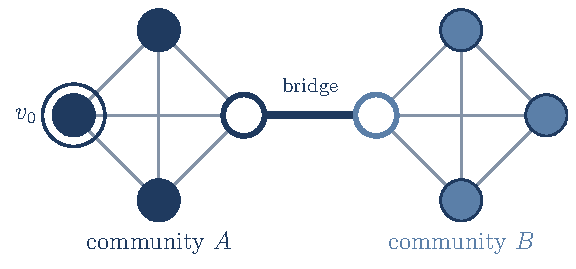
\includegraphics[width=0.9\linewidth]{images/barbell.pdf}\\
        {\small The barbell graph for \(k = 4\): everyone connected within a group of four, joined by one bridge; the message starts at \(v_0\).\par}
    \end{center}
}

\block{What the theory predicts}{
    The walk is irreducible (connected by the bridge) and aperiodic (by the triangles in \(K_k, \; k \geq 3\)). Detailed balance gives the stationary distribution (Lecture Notes, Ex.~7.13):
    \[\pi_v = \deg(v) / 2|E|, \quad |E| = k(k - 1) + 1\]
    \textbf{Crossing time:} The first time the message, started from \(v_0 \in A\), reaches \(B\). Let \(t_I\) and \(t_E\) be the expected times to reach \(B\) starting from an interior node and from the bridge node of \(A\). First-step analysis gives (Lecture Notes,~§7.4):
  \begin{align*}
    t_I &= 1 + \tfrac{k - 2}{k - 1}t_I + \tfrac{1}{k - 1}t_E \\[6pt]
    t_E &= 1 + \tfrac{k - 1}{k}t_I
  \end{align*}
  \[\implies \boxed{E[T_{\mathrm{cross}}] = t_I = k^2}\]

  \vspace{4mm}
  
  \textbf{Settling:} Let \(\Delta(n) = d_{\text{TV}}(P^n(v_0, \cdot), \pi)\) be the total variation distance from equilibrium. It drops within a few steps to about 0.5 (spreads quickly inside \(A\)), then it decays with rate \(|\lambda_2|\) per step, \(\lambda_2\) the second-largest eigenvalue of \(P\) (Lecture Notes, Theorem~7.8):
  \[\Delta(n) \approx \frac{1}{2}|\lambda_2|^{n}\]
  \innerblock{Theory, \(k = 4\)}{\centering \(E[T_{\mathrm{cross}}] = 16 \qquad  \lambda_2 = 0.887\)}
}

\column{0.5}

\block{Simulation against theory\strut}{
    \textbf{Crossing time}
    \begin{center}
        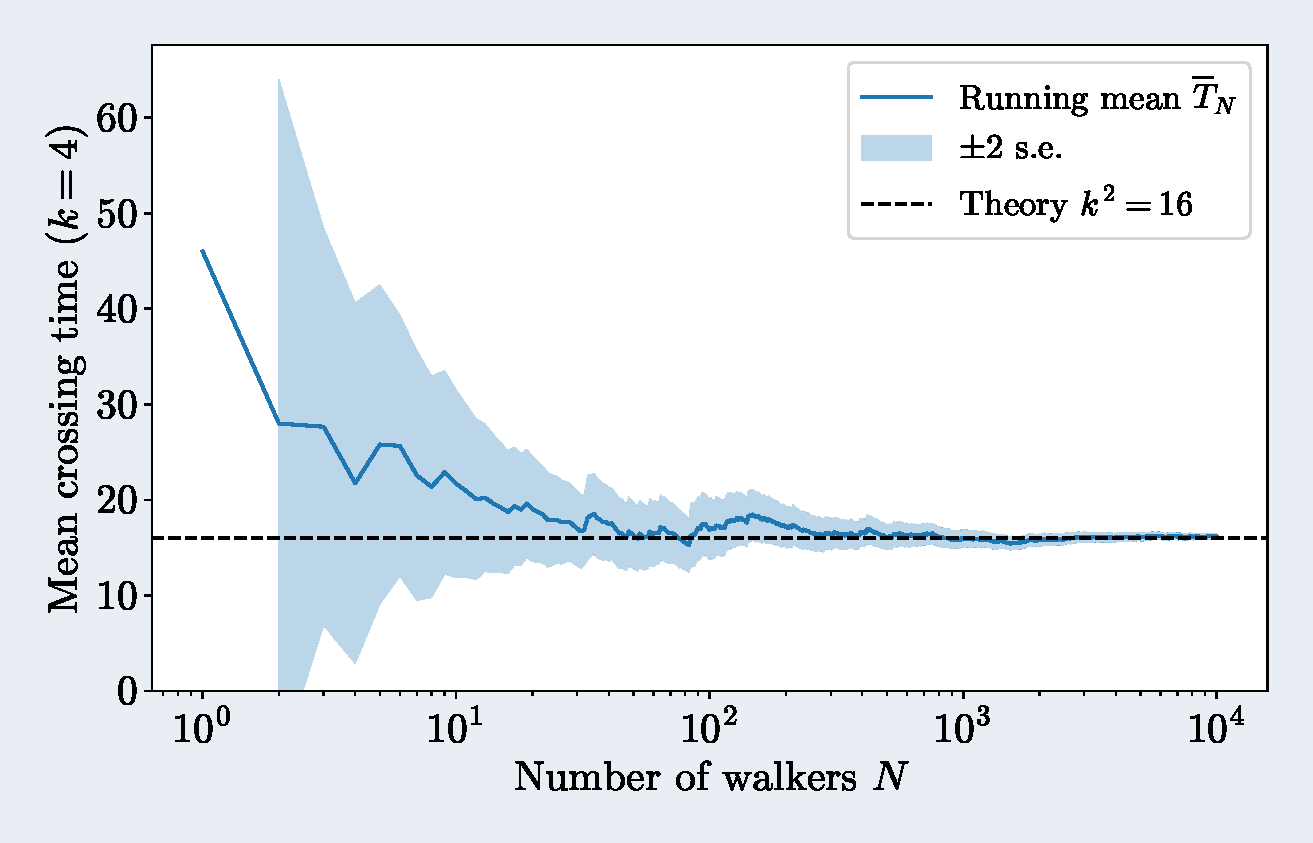
\includegraphics[width=0.95\linewidth]{images/cross_plot.pdf}\\[-6mm]
        {\small Running mean \(\overline{T}_N\) of the crossing time for \(k = 4\) approaches \(E[T_{\mathrm{cross}}] = k^2 = 16\) as the number of independent walkers \(N\) grows. The band is \(\pm2\)~s.e.\par}
  \end{center}
  \begin{center}\small
  \begin{tabular}{rcccc}
    \toprule
    $k$ & $N$ & Simulated $\overline{T}_N$ & Theory $k^2$ & Diff.\ (s.e.) \\
    \midrule
    \csname @@input\endcsname tables/table_cross
    \bottomrule
  \end{tabular}\\
  \vspace{4mm}
  Simulated \(\overline{T}_N\) against \(k^2\) for selected \(k\); Diff.\ is (simulated \(-\) theory) in standard errors, all falling within \(\pm 2\).
  \end{center}

  \textbf{Settling}
  \begin{center}
        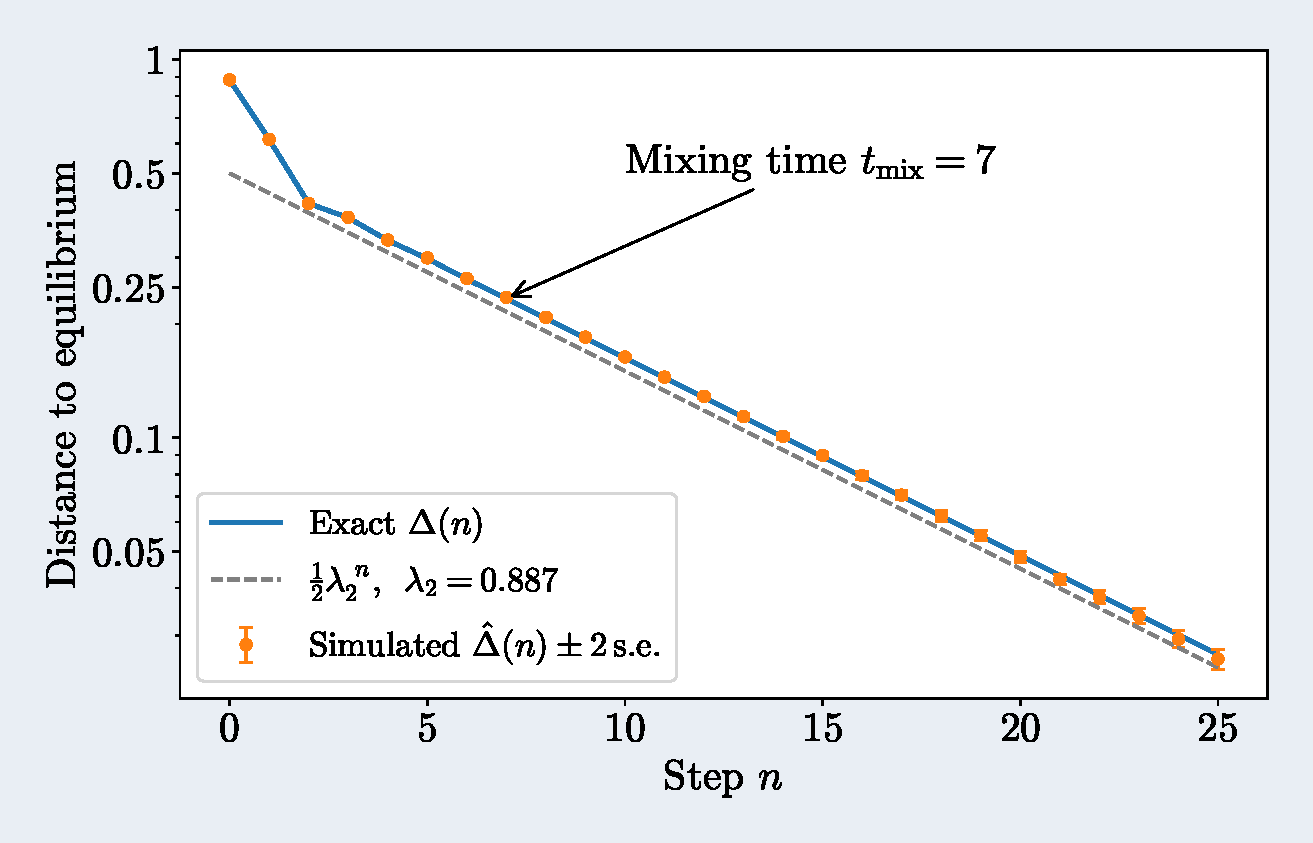
\includegraphics[width=0.95\linewidth]{images/dist_plot.pdf}\\[-6mm]
        % {\small Distance to equilibrium \(\Delta(n)\) for \(k = 4\): simulation (\(R = 30\) independent runs of \(N = 10^4\) walkers) matches the exact curve within 1~s.e.\ at every step and decays at rate \(\lambda_2 = 0.887\) as the theory predicted. \(t_{\mathrm{mix}} = 7\) is the first \(n\) with \(\Delta(n) \leq \tfrac{1}{4}\).\par}
        {\small Distance to equilibrium \(\Delta(n)\) for \(k = 4\): simulation (\(R = 30\) runs of \(N = 10^4\) walkers, \(\pm 2\)~s.e.\ whiskers) follows the exact curve and decays at rate \(\lambda_2 = 0.887\). \(t_{\mathrm{mix}} = 7\) is the first \(n\) with \(\Delta(n) \leq \tfrac{1}{4}\), the threshold of Levin et al.~(§4.5).\par}
  \end{center}
}

\block{What remains for the paper}{
  Check \(\pi(A) = \tfrac12\) from one long walk, with the s.e.\ by batch means; fit the decay to estimate \(\hat\lambda_2\) for each \(k\); explore the bias of the TV estimator near equilibrium.
  \vspace{1.4mm}
  }
\end{columns}

\node[anchor=south west, xshift=8mm, yshift=8mm, font=\small, text=black!60, text width=0.95\textwidth, align=left]
  at (bottomleft) {Sources: F.~Richter, \emph{Stochastic Methods: Lecture Notes}
  (2026); S.~M.~Ross, \emph{Introduction to Probability Models} (2019); D.~A.~Levin, Y.~Peres, E.~L.~Wilmer, \emph{Markov Chains and Mixing Times} (2017).};
\end{document}
